\documentclass{article}
\usepackage[utf8]{inputenc}
\usepackage{amsmath}
\newcommand{\dd}[1]{\mathrm{d}#1}
\usepackage{url}
\renewcommand{\refname}{Referencias}
\usepackage{float}

\title{Redes Neuronales \\
  \large Práctico 3 \\
  }
\author{Mariano Politano }
\date{Noviembre 2020}

\usepackage{natbib}
\usepackage{graphicx}

\begin{document}

\maketitle




En el presente práctico, trabajamos con un  \textbf{autoencoder} que es una red neuronal feed-forward. Utilizamos el conjunto de datos MNIST.
\\

A diferencia de un aprendizaje supervisado, donde se intenta predecir algo sobre la entrada, un \textbf{autoencoder} se utiliza para aprender una representación distribuida de nuestros datos de entrenamiento e incluso se puede utilizar para generar nuevas instancias de los datos de entrenamiento.  
En nuestro caso se utilizó para aprender la función identidad con la base de datos MNIST de dígitos escritos a mano y digitalizados. Este toma una imagen como entrada e intenta reconstruirla utilizando menos bits. 
La compresión en los \textit{autoencoder} se logra entrenando la red durante un periodo de tiempo.
En la figura \ref{figAuto} se puede observar un ejemplo simple de una red \textit{autoencoder}. En nuestro caso el input es de 784 neuronas  y la capa oculta (\textit{hidden}) es de 64 neuronas. (Luego, modificamos esta cantidad para ver como se comporta la red). El output tiene la misma cantidad de neuronas que el input.
\begin{figure}[H]
\centering
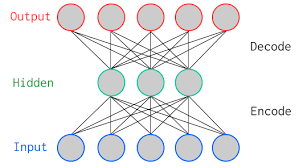
\includegraphics[width=7cm, height=4cm]{AutoEncoder.png}
\caption{Ejemplo simple de un autoencoder.}
\label{figAuto}
\end{figure}
Un modelo \textit{feed-forward autoencoder} contiene dos componentes:

\begin{itemize}
\item Un codificador que toma una imagen como entrada y genera una representación de baja dimensión de la imagen.
\item Un decodificador que toma la incrustación de baja dimensión y reconstruye la imagen. 
\end{itemize}

En nuestro práctico, las imágenes tiene un tamaño de 28 x 28 píxeles en escalad de grises. El dataset tiene 60000 imágenes en el conjunto de entrenamiento y 10000 imágenes en el conjunto de test.
En la \ref{fig1} se puede ver algunos ejemplos del dataset.
\begin{figure}[H]
\centering
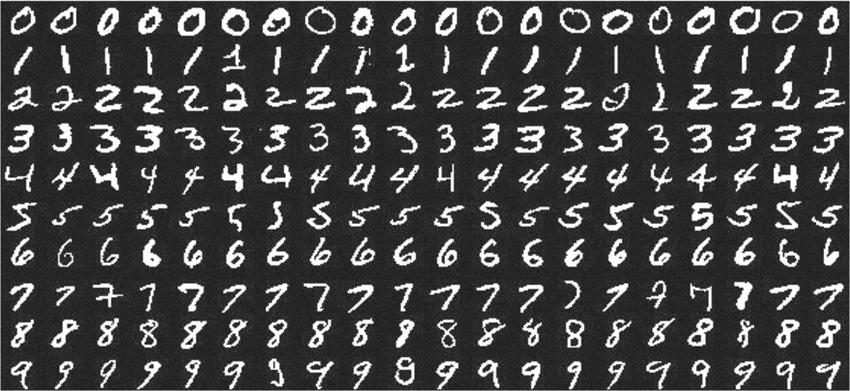
\includegraphics[width=\textwidth]{example.png}
\caption{Dataset de MNIST.}
\label{fig1}
\end{figure}




\section*{Resolución}

Para trabajar con el dataset, se transformaron las entradas de las imágenes de 28 x 28 píxeles a vectores de 784 dimensiones. Luego estos son pasados por una capa densa (Fully-Connected) con función de activación ReLU para generar una representación interna de 64 dimensiones. Finalmente el flujo sigue a una capa de salida con 784 neuronas para reconstruir la entrada con función de activación ReLU.
La red se entreno durante 15 épocas. Como optimizador se utilizo Adam (Adaptive Moment Estimation) con una taza de aprendizaje de $0.001$, con dropout de $p= 0.1$ y minibatch de tamaño 1000.
\\

En la figura \ref{fig1} se puede ver que la función de pérdida a lo largo de las épocas decrece en ambas curvas, motivo por el cual se puede descartar un overfitting. Y por ende, se puede ver que a lo largo de las épocas la red mejora y tiene menos perdida, lo que significa que obtiene buenas soluciones candidatas.

\begin{figure}[H]
\centering
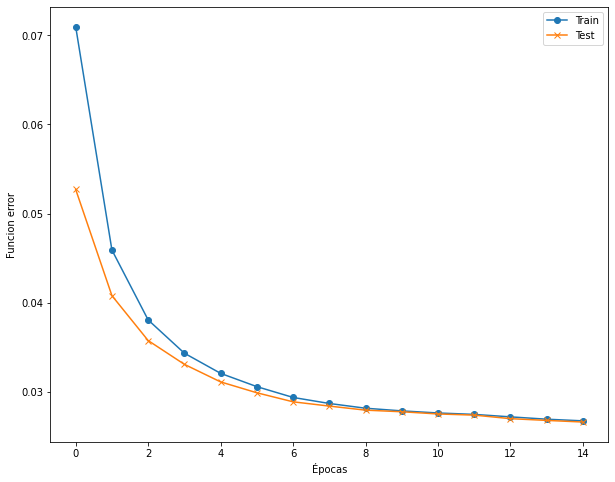
\includegraphics[width=\textwidth]{Train-vs-test.png}
\caption{Función error en train y test en base de las épocas. 64 neuronas internas }
\label{fig1}
\end{figure}

En la figura \ref{fig3} se puede observar una reconstrucción de la entrada generada por la red.

\begin{figure}[H]
\centering
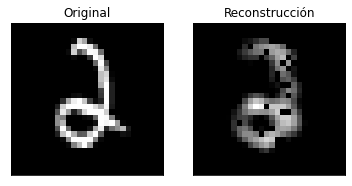
\includegraphics[width=7cm, height=4cm]{examples2.png}
\caption{Reconstrucción generada por la red. }
\label{fig3}
\end{figure}

Luego se modifico la cantidad de neuronas en la capa oculta, tomando los valores de 64, 128, 256 y 512. Los resultados de como se comporta la función de perdida a lo largo de las épocas durante el entrenamiento y la validación se pueden ver en la figura \ref{fig5}

\begin{figure}[H]
\centering
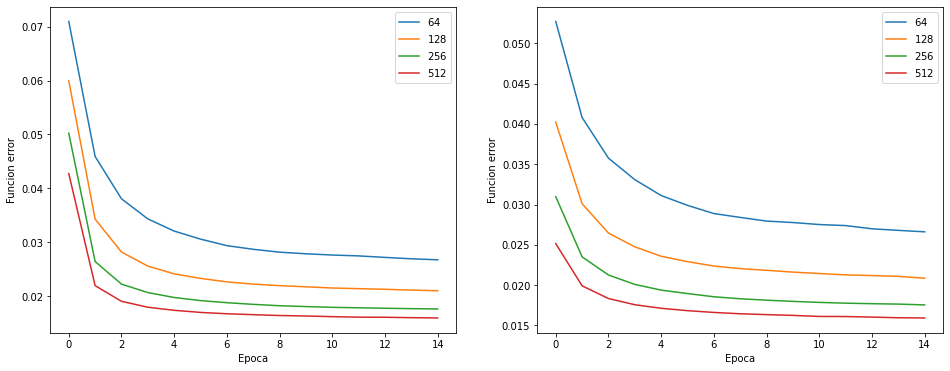
\includegraphics[width=\textwidth]{graficoDiferente.png}
\caption{Función de perdida para distintos valores de capa ocultas. A la izquierda durante el entrenamiento, a la derecha durante la validación }
\label{fig5}
\end{figure}

Podemos concluir que las redes autoencoder son útiles para obtener representaciones de baja dimensionalidad lo que permite ahorrar espacio de almacenamiento y computo.

\\
\


\textbf{Nota}: El práctico fue realizado en \textit{Python}, con ayuda de Gooogle Colab y se utilizo la librería Torch como se vio en clases.
    

\bibliographystyle{plain}
\bibliography{Referencias}
\begin{itemize}


\item Pizarrones de clases

\item \url{https://www.datacamp.com/community/tutorials/autoencoder-keras-tutorial#autoencoders}
\item \url{https://www.inteldig.com/2018/05/tutorial-pytorch-aprendizaje-profundo-deep-learning-en-python/}
\item \url{https://towardsdatascience.com/how-to-make-an-autoencoder-2f2d99cd5103}

\item Código del práctico:  \url{https://github.com/mpolitano/redesNueronales/ }

\end{itemize}

\end{document}